\documentclass{article}

\usepackage[francais]{babel}
\usepackage[T1]{fontenc}
\usepackage{geometry}
\geometry{hmargin=2.5cm}
\usepackage{amsmath}
\usepackage{graphicx}
\usepackage{subcaption}
\usepackage{float}
\usepackage{hyperref}
\usepackage{setspace}
\usepackage{xcolor}
\usepackage{pdfpages}
\usepackage{enumitem}
\usepackage{lscape}

\title{Jeu awélé\bigbreak \bigbreak
    \large Analyse UML}

\date{20 mai 2020}
\author{Laura Binacchi}

\begin{document}
    \pagenumbering{gobble}
    
\includepdf[pages={1}]{pdg}
    \newpage
    \tableofcontents
    \newpage
    \pagenumbering{arabic}

    \section*{Introduction}
    \label{sec:intro}
    \addcontentsline{toc}{section}{\nameref{sec:intro}}

    \paragraph{}
    Ce travail présente l'analyse UML du jeu awélé réalisée dans le cadre du cours de Programmation orientée objet. L'awélé est un jeu de semailles d'origine africaine dont le but est de récolter le maximum de graines sur un plateau composé de 12 trous. Les règles de ce jeu sont détaillées dans la première section de ce travail.

    \paragraph{}
    La première version de ce jeu sera une application en console codée en Java. Le joueur jouera face à la machine en mode facile (aléatoire) ou difficile (intelligence artificielle). Cette analyse présente la première version du jeu avec la machine en mode aléatoire.

    \paragraph{}
    La deuxième version du jeu consistera à ajouter une interface graphique avec JavaFX. Pour cette raison, la première version du jeu se concentrera sur la partie logique et non sur les fonctionnalités graphiques et d'interaction avec l'utilisateur.  

    \paragraph{}
    La troisième et dernière version ajoutera une fonctionnalité permettant d'enregistrer un score et d'afficher le tableau reprenant les meilleurs scores en liant l'application à une base de données.
    
    \paragraph{}
    Après avoir présenté les règles du jeu awéle, je présenterai le diagramme de cas d'utilisation de l'application. Je présenterai ensuite un schéma de classes simplifié qui se concentre sur la logique du jeu et un schéma détaillé reprenant l'intégralité des classes implémentées dans la première version avec leurs champs et méthodes. Enfin, je présenterai une succession de diagrammes de séquence permettant de comprendre les interactions entre les différents éléments du jeu.

    \newpage
    \section{Règles du jeu awélé}

    \paragraph{}
    Le jeu awélé est un jeu de semailles qui se joue à 2 joueurs.     Le jeu se compose d'un plateau à 12 trous et de 48 graines. Les trous sont organisés en 2 rangées de 6, chacune appartenant à un joueur : joueur 1 (orange) et joueur 2 (bleu). Le but est de récolter le maximum de graines : le joueur qui en comptabilise plus de 24 gagne la partie.

    \begin{figure}[H]
        \centering
        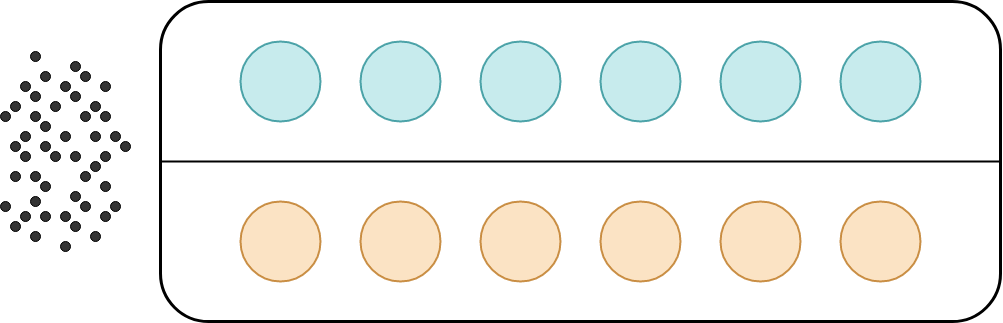
\includegraphics[width=.55\linewidth]{./images/rules-composition.png}
        \caption{Composition du jeu : plateau à $2 \times 6$ trous et 48 graines}
    \end{figure}

    \paragraph{}
    Au début du jeu, 4 graines sont placées dans chaque trou. Les joueurs se trouvent de part et d'autre du plateau, face à leur rangée de graines. Tour à tour, chacun va semer ses graines et tenter d'en récolter. 
    
    \paragraph{}
    A chaque tour, le joueur saisit les graines se trouvant dans l'un de ses trous et les sème une par une dans les trous suivants (dans le sens antihoraire), y compris dans ceux de son adversaire et à l'exception du trou de départ (s'il sème plus de 11 graines, il devra sauter le trou de départ et continuer à partir du suivant).

    \begin{figure}[H]
        \centering
        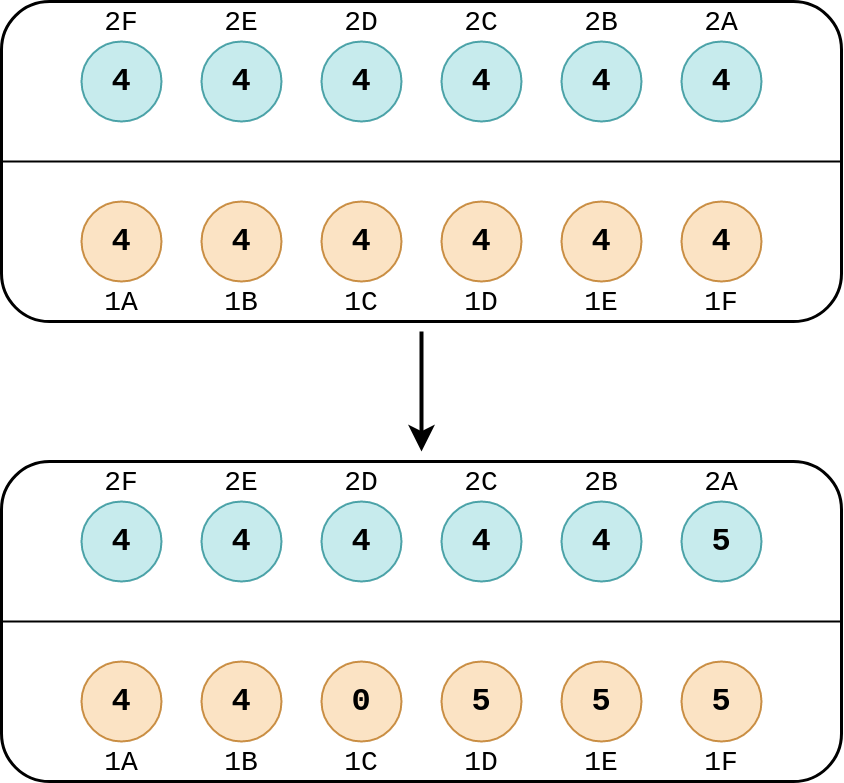
\includegraphics[width=.55\linewidth]{./images/tour1.png}
        \caption{Premier tour : le joueur 1 sème les graines de la case C}
    \end{figure}

    \paragraph{}
    Si la dernière graine est semée dans un des trous adverses et que ce dernier comptait 1 ou 2 graines avant le semis, le joueur prend le contenu de ce trou. Si le trou précédent compte lui aussi 2 ou trois graines après le semis, le joueur peut également les récolter et ainsi de suite. La récolte s'arrête dès que le joueur tombe sur un trou qui compte plus de 3 graines ou s'il revient à la première case adverse.

    \begin{figure}[H]
        \centering
        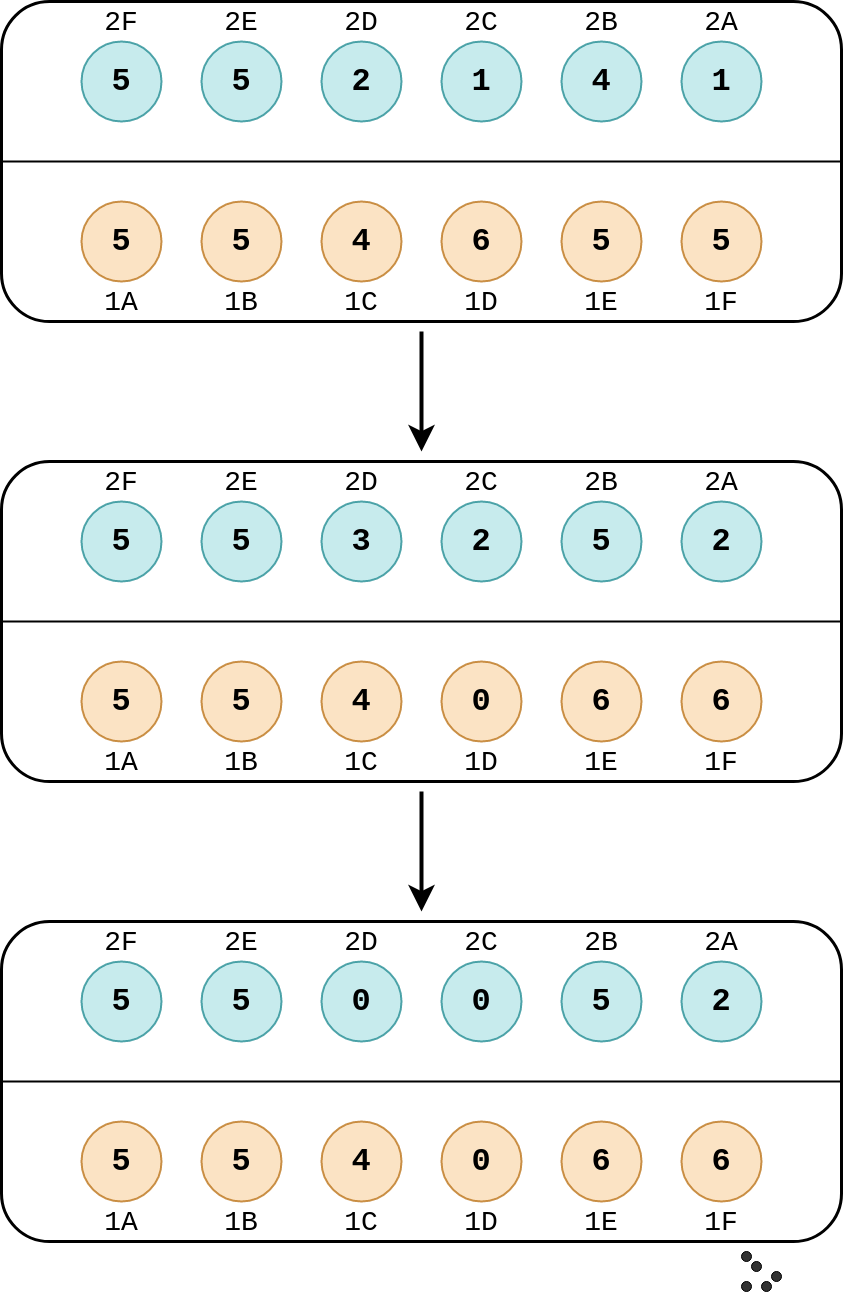
\includegraphics[width=.55\linewidth]{./images/recolte1.png}
        \caption{Le joueur 1 sème les graines de la case D et récolte 5 graines}
    \end{figure}
    
    \paragraph{}
    Il est obligatoire de nourrir l'adversaire : si un des joueurs se retrouve sans graines, l'autre doit à son tour semer des graines dans les cases adverses.

    \paragraph{}
    Il est interdit d'affamer l'adversaire : la rangée d'un joueur ne peut pas être entièrement récoltée par son adversaire. Si un semis entraîne une récolte qui affame l'adversaire, cette récolte ne peut pas se faire.

    \paragraph{}
    La partie peut s'arrêter dès que l'un des deux joueurs a récolté plus de 24 graines mais elle peut aussi continuer pour compter les points.
    
    \paragraph{}
    La partie s'arrête obligatoirement dès qu'il est impossible pour un des joueurs de nourrir l'adversaire affamé : ce joueur peut alors récolter les graines qui se trouvent encore sur sa rangée et le joueur qui comptabilise alors le plus de graines en réserve gagne la partie.

    \paragraph{}
    Une partie s'achève toujours sur l'un des trois cas suivants : le premier joueur gagne, le second joueur gagne, ou il y a match nul.


    \newpage
    \section{Diagramme de cas d'utilisation}

    \paragraph{}
    Ce diagramme expose les cas d'utilisation du jeu \textbf{AWELE} par un \textbf{joueur} :
    \begin{itemize}
        \item Jouer une partie
        \item Choisir la difficulté
        \item Enregistrer un score
        \item Consulter les scores
    \end{itemize}

    \begin{figure}[H]
        \centering
        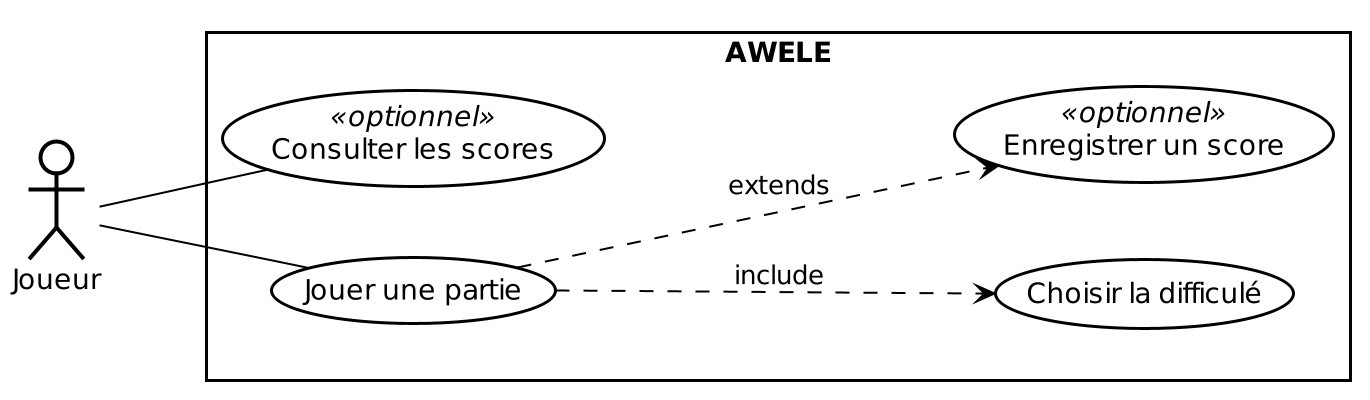
\includegraphics[width=.75\linewidth]{./schemas/usecase.png}
        \caption{Diagramme de cas d'utilisation}
    \end{figure}

    \paragraph{}
    La cas d'utilisation principal est évidemment de \textbf{jouer une partie}. Jouer une partie suppose de \textbf{choisir la difficulté} de celle-ci (relation d'inclusion) : à chaque fois que le joueur lance une nouvelle partie, le jeu lui demande s'il souhaite jouer en mode normal ou difficile.

    \paragraph{}
    En fin de partie et selon certaines conditions, le  joueur pourra ou non \textbf{enregistrer son score} (relation d'extension).

    \paragraph{}
    Le joueur aura enfin la possibilité de consulter les scores précédemment enregistrés. Cette fonctionnalité sera développée dans la troisième version du projet avec l'implémentation d'une liaison avec une base de données locale.

    \newpage
    \section{Diagramme de classes simplifié : logique du jeu}
    \paragraph{}
    Ce diagramme présente une première modélisation de la logique du jeu dans la première version développée : le joueur joue face à un joueur virtuel en mode facile et l'enregistrement des scores n'est pas encore possible.

    \begin{figure}[H]
        \centering
        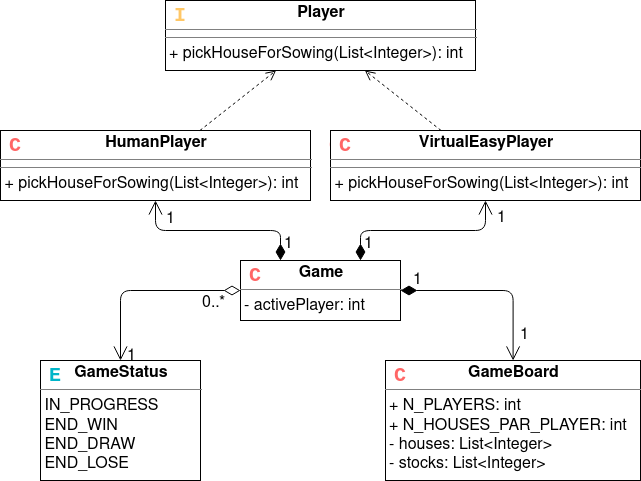
\includegraphics[width=0.7\linewidth]{./schemas/classes1.png}
    \end{figure}

    \paragraph{}
    La classe centrale est la classe \textbf{Game} qui centralise un \textbf{GameBoard} et deux joueurs implémentant l'interface \textbf{Player} : un joueur humain \textbf{HumanPlayer} et un joueur virtuel en mode facile \textbf{VirtualEasyPlayer}. C'est une relation de composition car il n'est pas prévu d'enregistrer un jeu ou un joueur. Le jeu stocke également un entier correspondant au joueur actif \textbf{activePlayer} et un statut de type \textbf{GameStatus} qui sert à déterminer si le jeu est en cours ou fini et de quelle manière (le joueur humain a gagné, perdu, ou fait match nul).

    \paragraph{}
    Pour compléter le jeu, d'autres classes doivent être ajoutées pour gérer l'affichage du plateau de jeu et des messages destinés au joueur et pour gérer la navigation dans les menus et la dynamique du jeu. C'est ce que présente le diagramme de classes suivant.

    \newpage
    \section{Diagramme de classes détaillé}
    \begin{figure}[H]
        \centering
        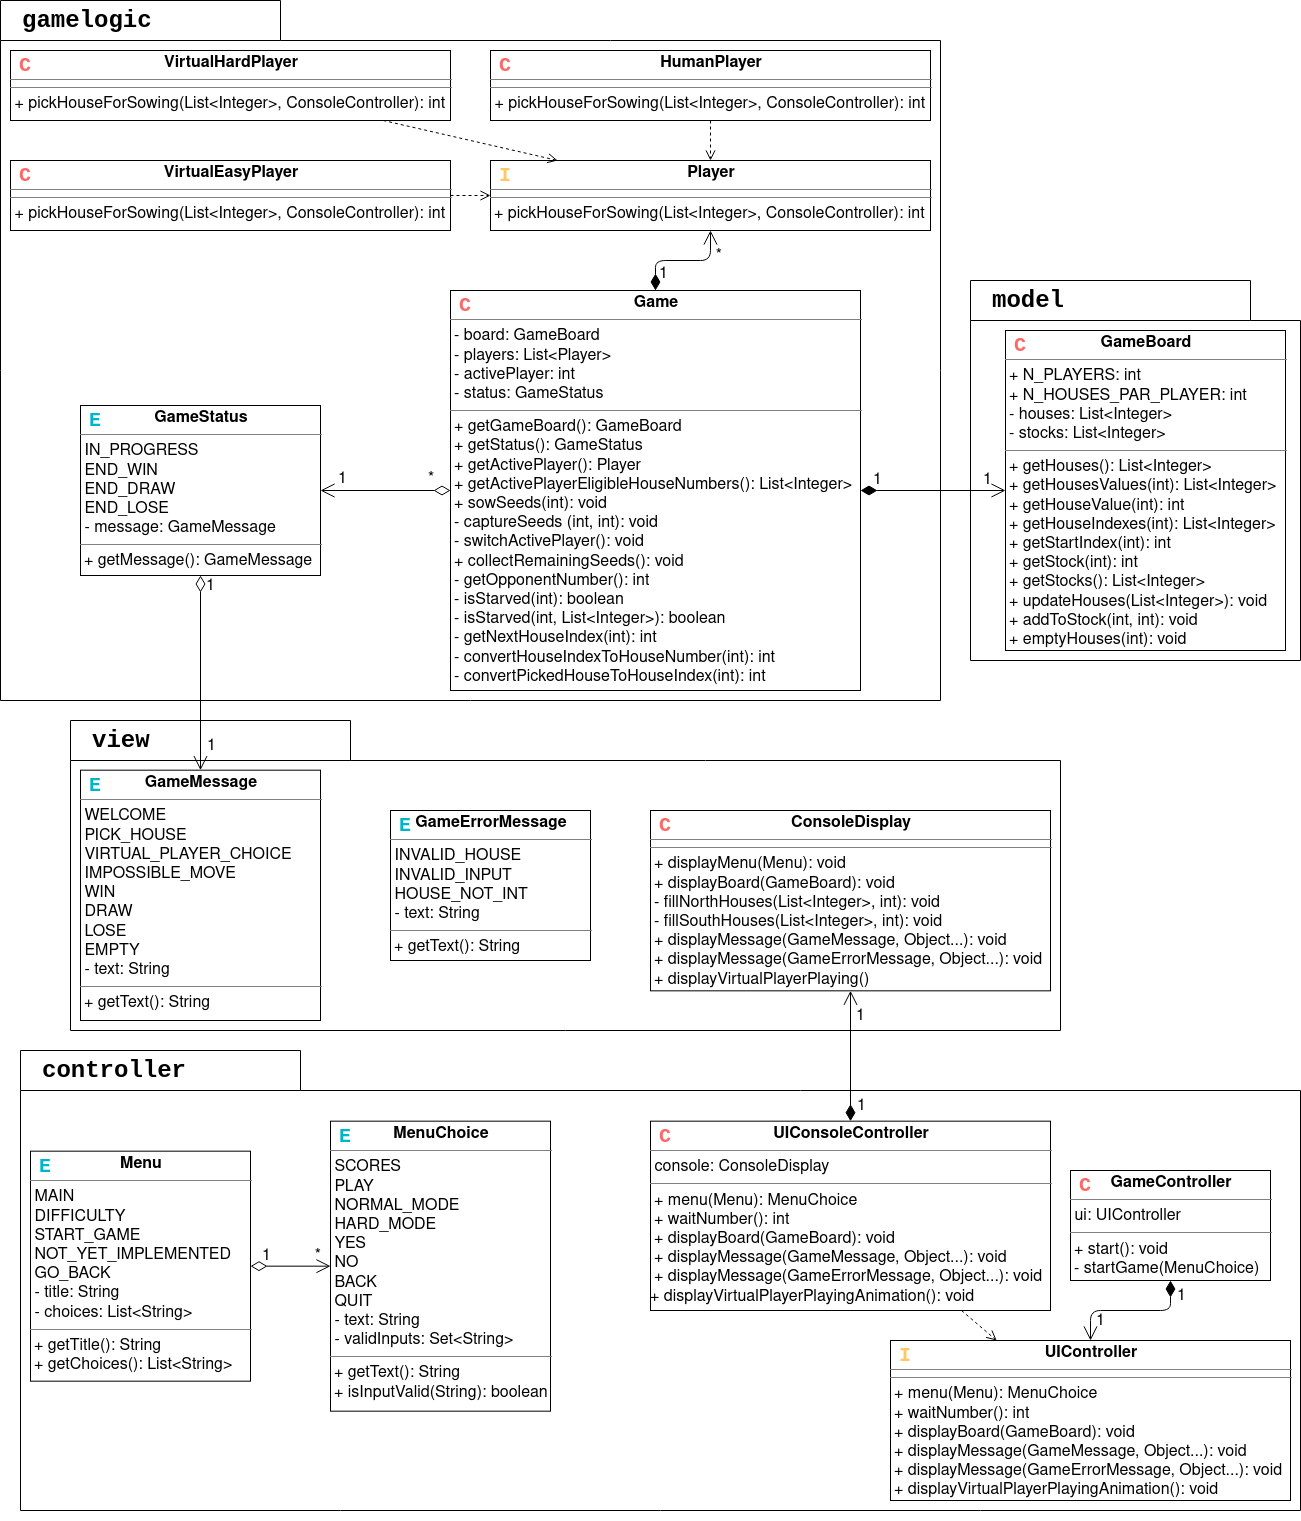
\includegraphics[width=0.94\linewidth]{./schemas/classes2.png}
    \end{figure}

    \paragraph{}
    Ce diagramme présente l'ensemble des classes avec champs et méthodes à implémenter pour réaliser la première version du jeu. Les classes de la logique du jeu présentées dans la section précédente sont regroupées dans la package \textbf{gamelogic} qui rassemble les classes de contrôle du jeu et des joueurs qui pourront être réutilisées pour toutes les versions futures du jeu.

    \paragraph{}
    La classe représentant le plateau de jeu a été séparée dans la package \textbf{model}. Cette classe reprend les données du jeu et les méthodes pour y accéder et les modifier. Lorsque l'enregistrement des scores sera implémenté dans la troisième version du jeu, c'est également dans ce package que sera placée la classe \textbf{Score}.

    \paragraph{}
    Le package \textbf{view} sépare les classes qui sont propres à l'affichage : les messages et messages d'erreur et les appels au système pour l'affichage en console. Les messages affichés seront conservés mais la manière dont ils seront affichés sera implémentée différemment dans la version suivante du jeu. Les menus sont écrits de manière déclarative pour faciliter les changements futurs.

    \paragraph{}
    Enfin le package \textbf{controller} reprend les classes de contrôle du jeu. Le \textbf{GameController} gère la navigation dans les menus et le démarrage d'un nouveau jeu. A sa création, une classe implémentant l'interface \textbf{UIController} lui est donnée : elle permet de gérer l'arrivée des inputs du joueur (choix des menus ou sélection d'un nombre durant le jeu) et d'appeler la vue pour l'affichage des messages et du plateau de jeu. Dans la première version du jeu, c'est la classe \textbf{UIConsoleController} qui implémente cette interface. Dans la seconde, ce sera une classe JavaFX.


    \newpage
    \section{Diagramme de séquence système}
    \begin{figure}[H]
        \centering
        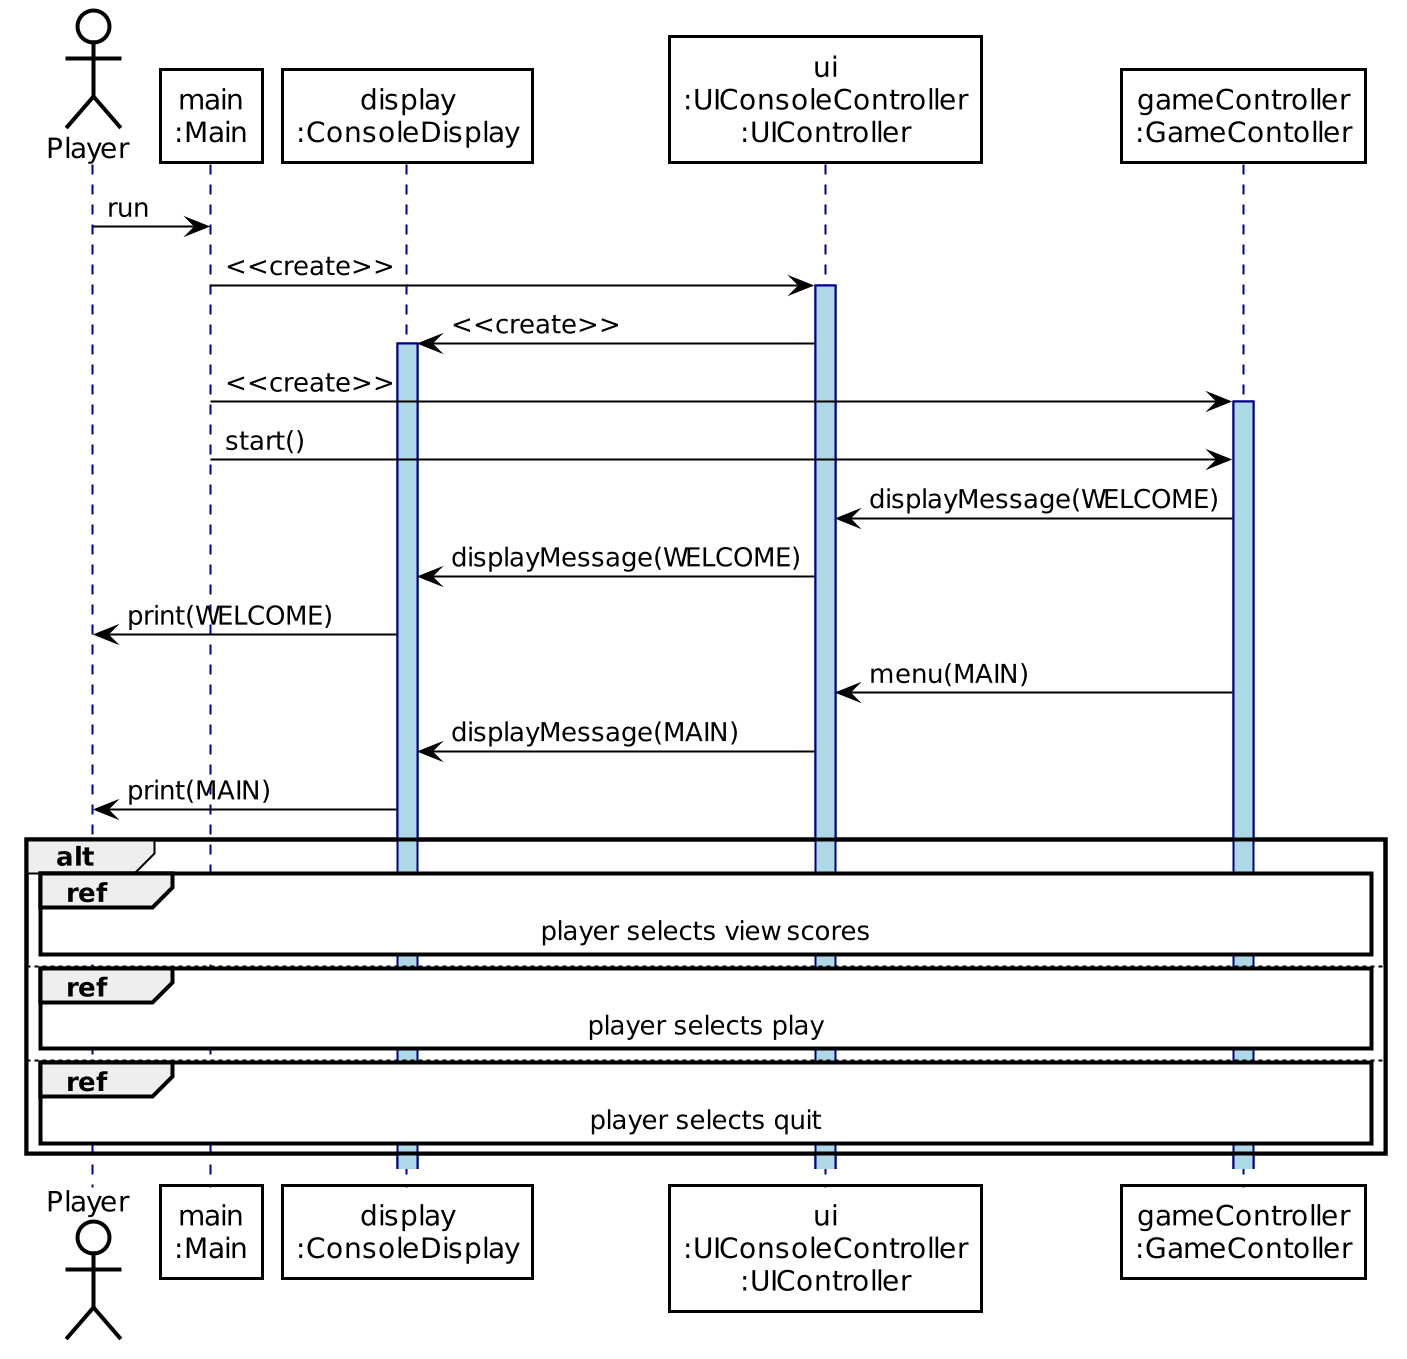
\includegraphics[width=.8\linewidth]{./schemas/sequence1-overview.png}
    \end{figure}

    \paragraph{}
    Ce diagramme présente le fonctionnement global de l'application avec les références aux diagrammes de séquences dont certains sont développés dans les sections suivantes.

    \paragraph{}
    Lorsque le joueur lance l'application, une instance du \textbf{GameController} et une instance du \textbf{UIController} sont créées, ainsi qu'une instance du \textbf{ConsoleDisplay} qui dépend du \textbf{UIConsoleController}. Ces instances sont les seules crées par le programme, ce sont donc des Singleton. Leur durée de vie s'étend sur toute la durée de vie de l'application.

    \paragraph{}
    Le menu principal du jeu permet de consulter les scores (à implémenter dans la version 3), de jouer ou de quitter l'application. Le diagramme suivant développe la séquence où le joueur sélectionne l'option "jouer".


    \newpage
    \section{Diagramme de séquence : le joueur choisit le menu "jouer"}

    \begin{figure}[H]
        \centering
        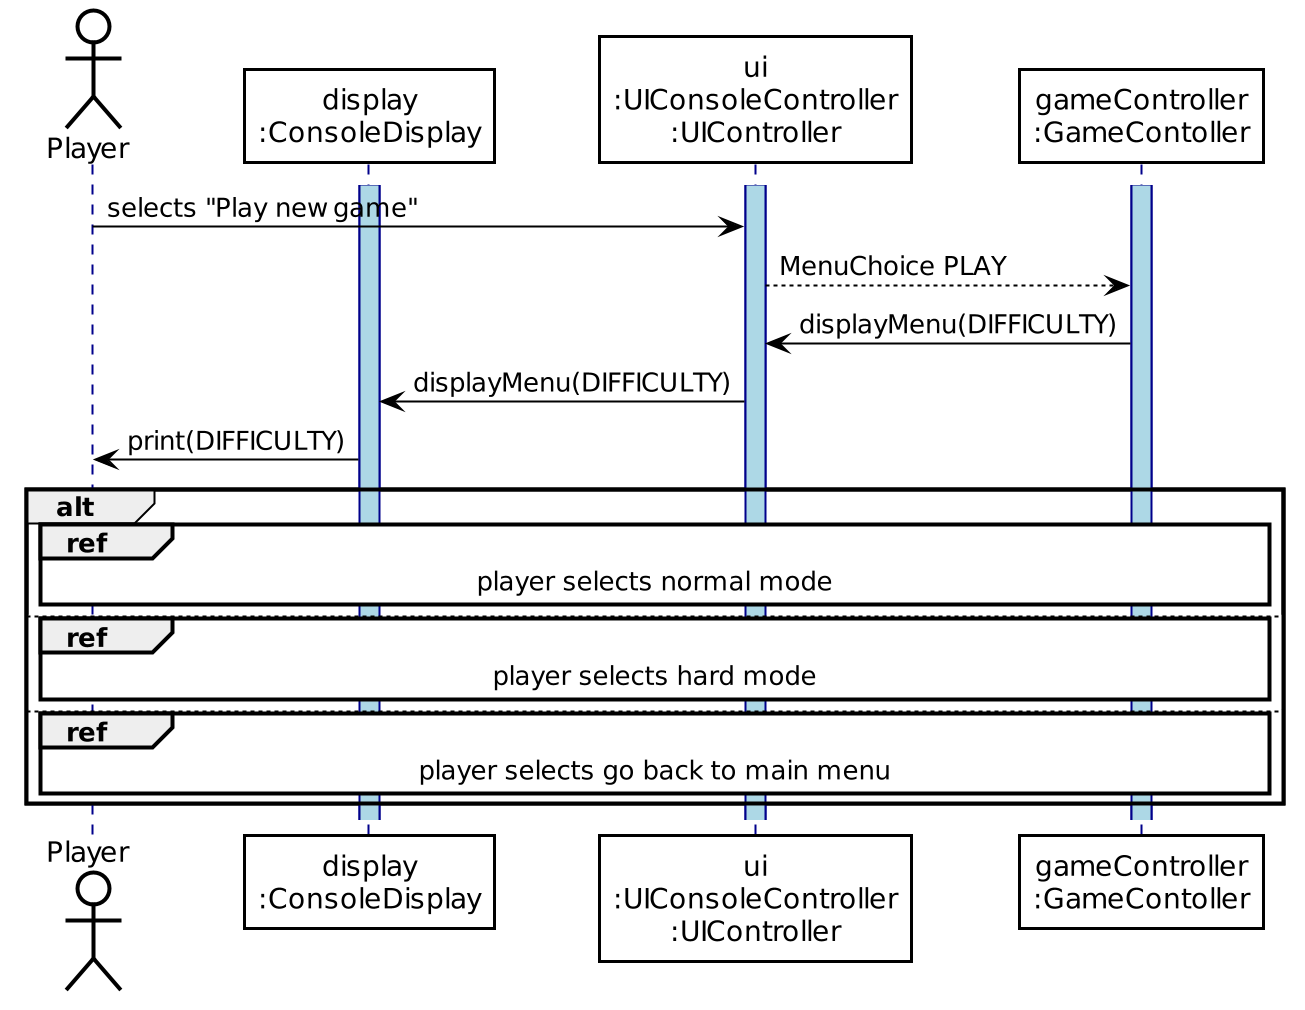
\includegraphics[width=.8\linewidth]{./schemas/sequence2-player-selects-play.png}
    \end{figure}

    \paragraph{}
    Lorsque le joueur sélection le menu "jouer", il doit choisir entre le mode normal (le joueur virtuel joue en mode aléatoire) ou le mode difficile. Il peut aussi choisir de revenir au menu principal. Le diagramme suivant présente la séquence où le joueur choisit de jouer en mode normal.


    \newpage
    \section{Diagramme de séquence : le joueur choisit le mode normal}

    \begin{figure}[H]
        \centering
        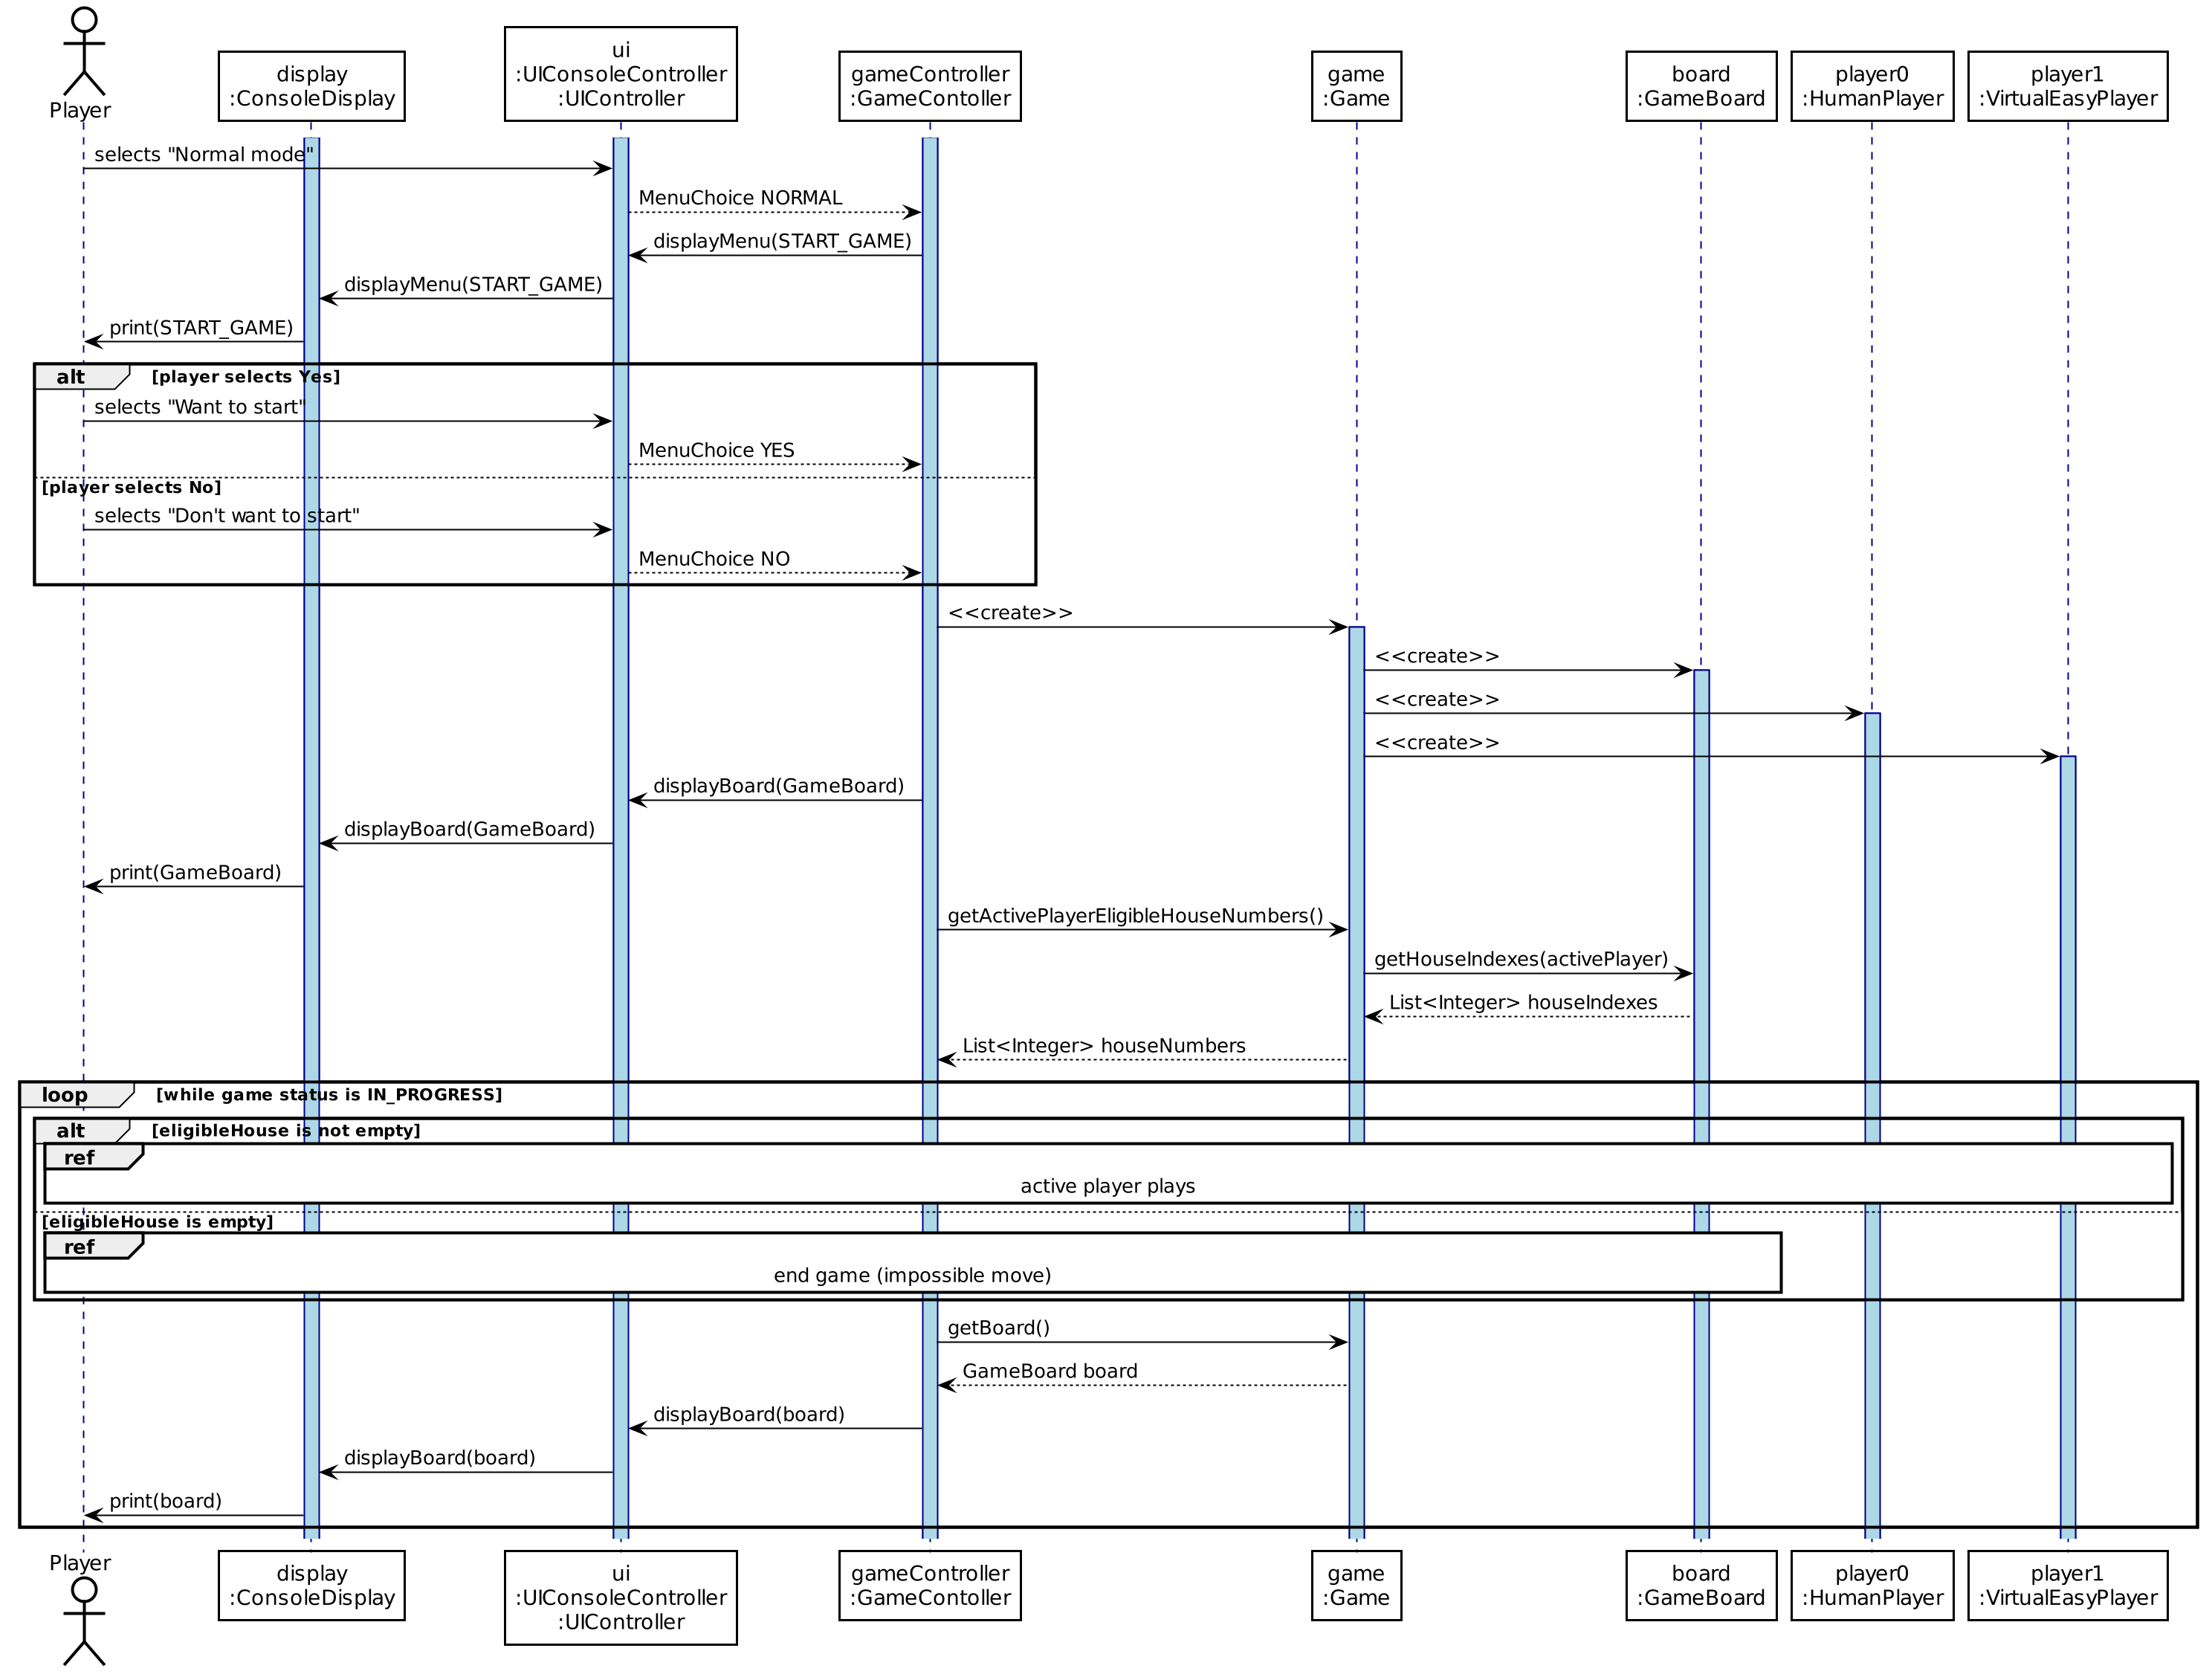
\includegraphics[width=\linewidth]{./schemas/sequence3-player-selects-normal.png}
    \end{figure}

    \paragraph{}
    Lorsque le joueur a choisi la difficulté du jeu, il doit choisir s'il souhaite commencer la partie ou si c'est le joueur virtuel qui commence. Ce choix déterminera la variable \textbf{activePlayer} de la classe \textbf{Game}.

    \paragraph{}
    Le contrôleur du jeu peut alors créer un nouveau jeu dont les paramètres dépendent des choix de l'utilisateur. Ce nouveau jeu crée un plateau qui lui est associé et deux joueurs : le joueur humain (\textbf{player0}) et le joueur virtuel (\textbf{player1}). Ces entités seront détruites au moment où le jeu prendra fin.

    \paragraph{}
    Tant que le jeu est en cours, i.e. tant que son statut n'a pas définit de gagnant, les tours de jeu s'enchaînent de la manière suivante : le contrôleur récupère la liste des trous qui peuvent être joués par le joueur actif. Si cette liste est vide, le jeu se termine car plus aucun mouvement n'est possible. Sinon, le joueur actif joue. Ces deux séquences sont présentées dans les deux derniers diagrammes de ce travail.

    \newpage
    \section{Diagramme de séquence : le joueur actif joue}

    \begin{figure}[H]
        \centering
        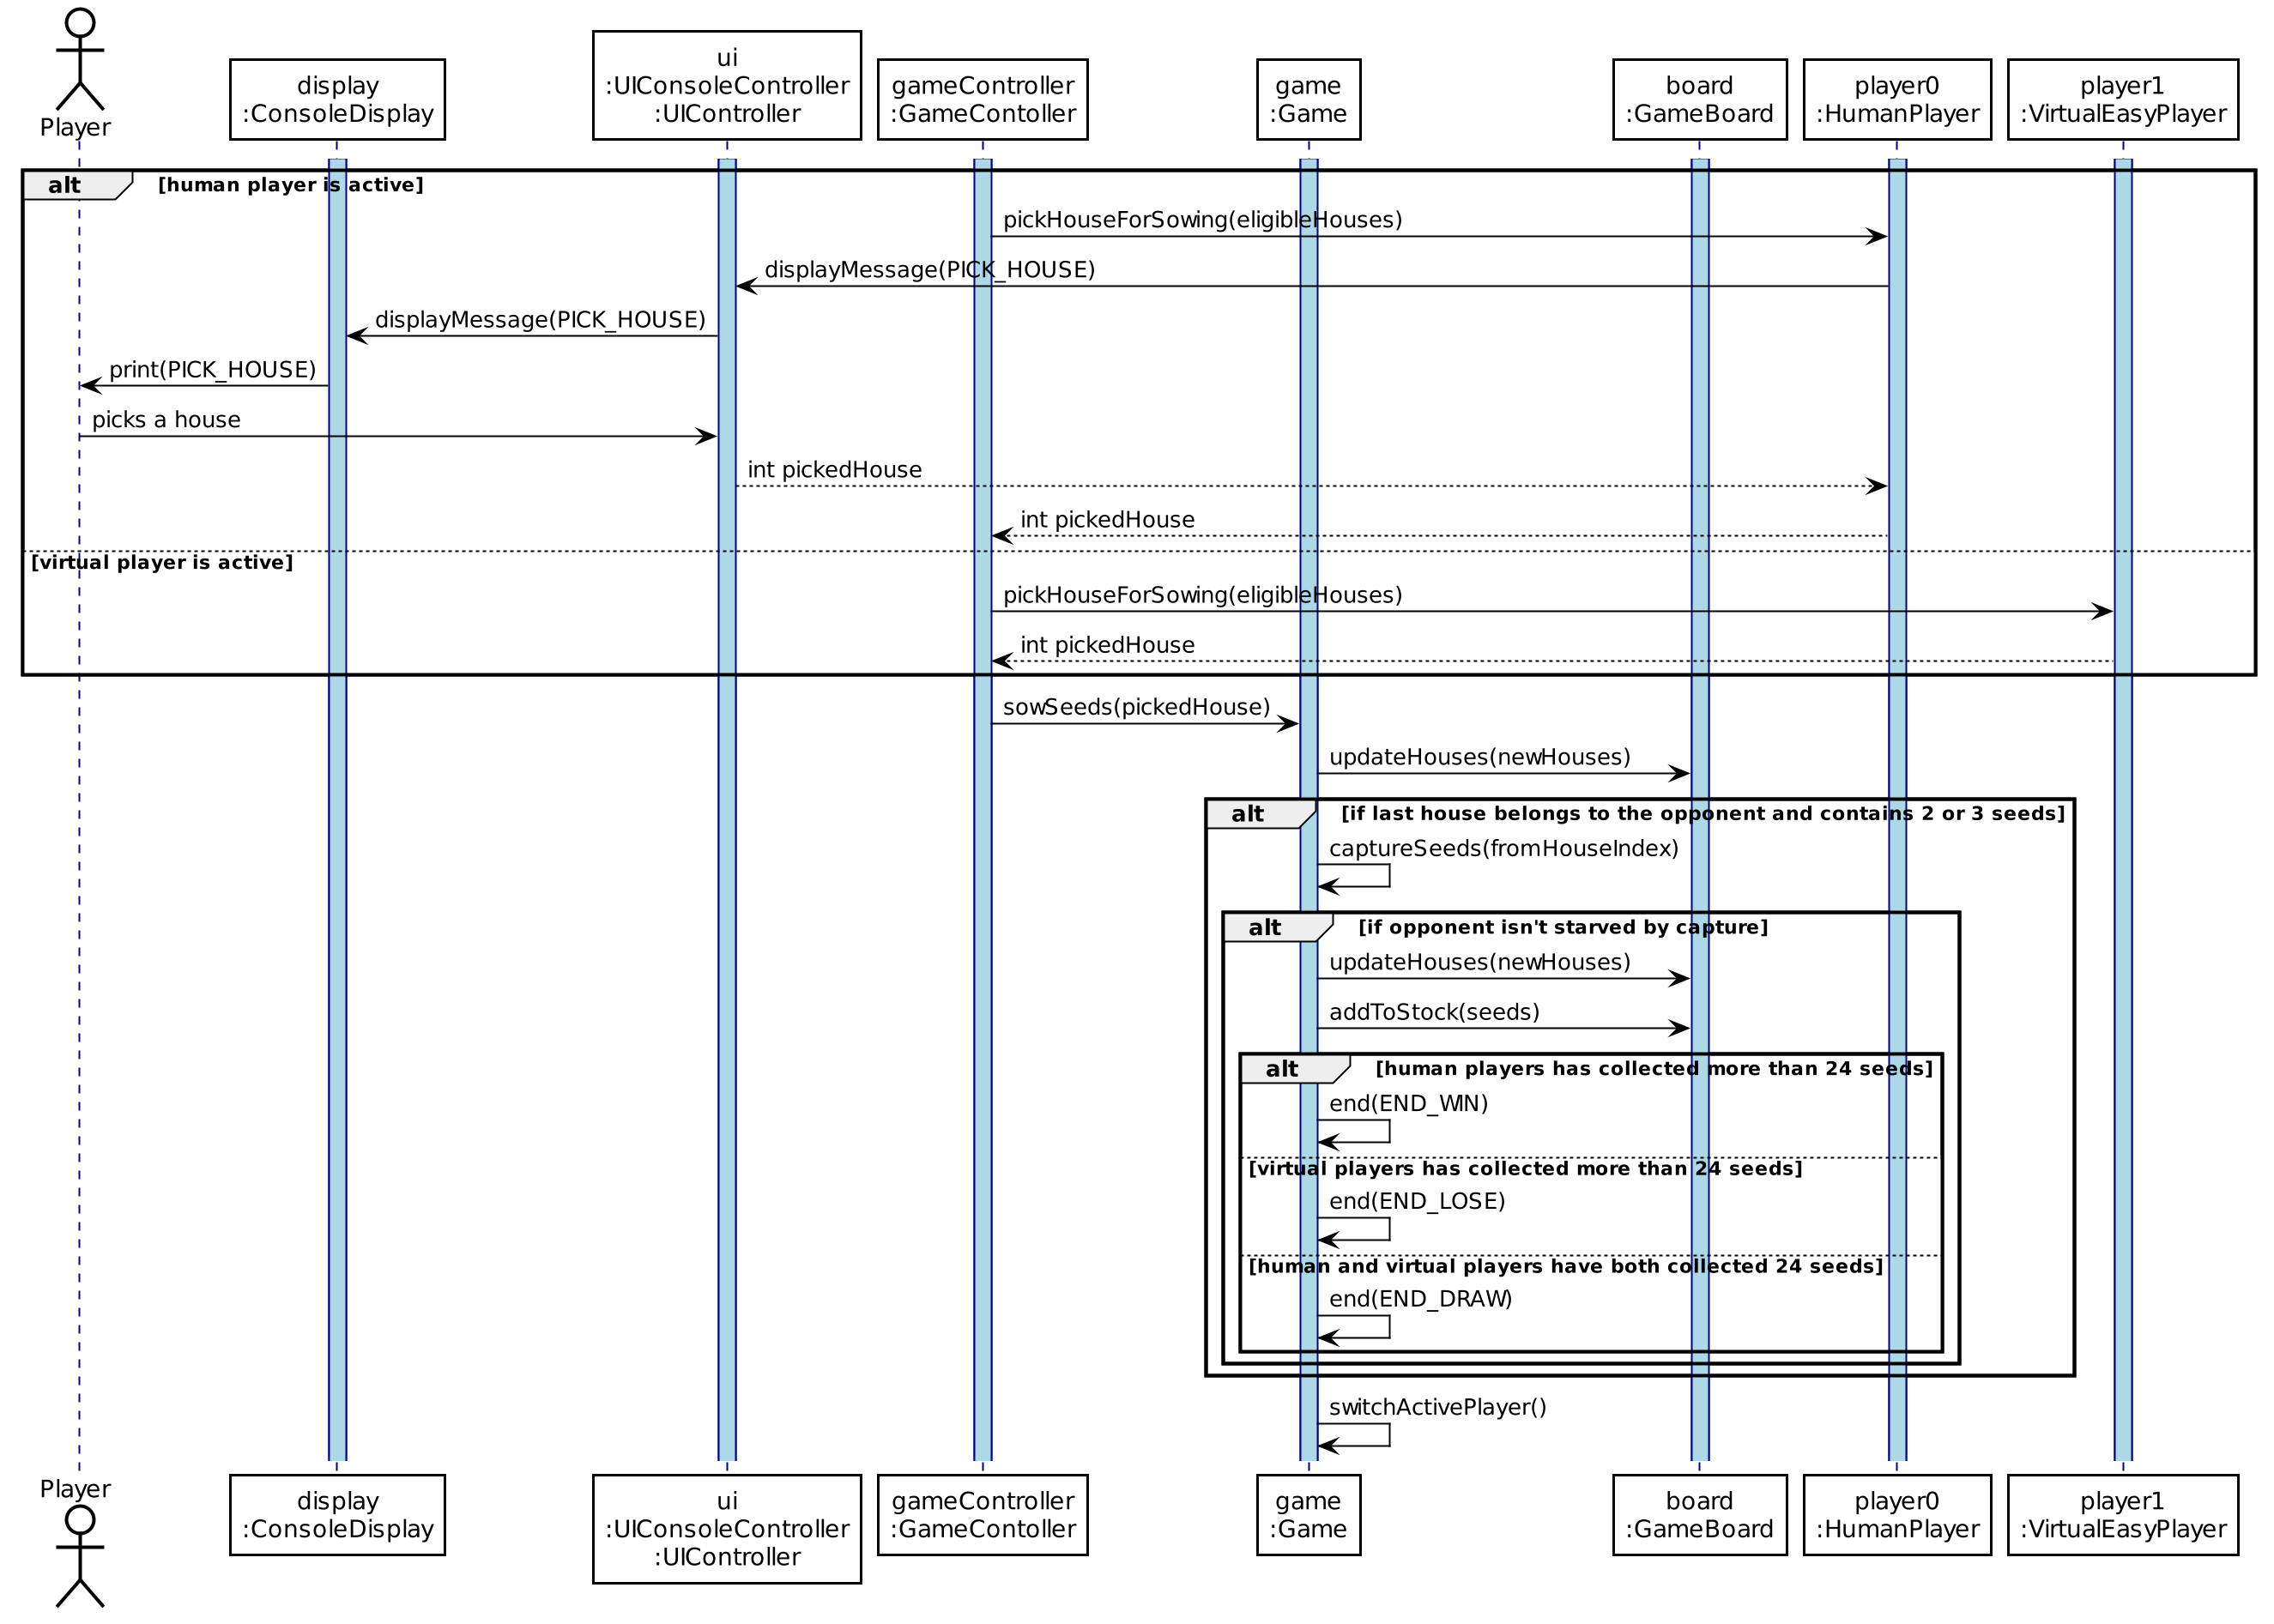
\includegraphics[width=\linewidth]{./schemas/sequence4-active-player-plays.png}
    \end{figure}

    \paragraph{}
    Si c'est le joueur humain qui est actif, le contrôleur du jeu doit faire appel au contrôleur de l'interface utilisateur pour lui demander de choisir un trou à jouer parmi la liste des numéros valides. Si c'est un joueur virtuel, la même méthode est appelée chez lui pour choisir un trou dans la liste des nombres valides.

    \paragraph{}
    Les graines sont ensuite semées dans les trous suivant et si le dernier trou appartient à l'adversaire et contient deux ou trois graines, elles sont capturées. Si la capture n'affame pas l'adversaire, elle est validée et la réserve du joueur est mise à jour.

    \paragraph{}
    Lorsqu'une réserve est mise à jour, le jeu vérifie si l'une des deux réserves comporte plus de 24 graines. Le jeu peut alors se terminer en définissant le gagnant ou sur un match nul dans le cas où les deux joueurs ont récolté chacun 24 graines.

    \paragraph{}
    Enfin, le joueur actif est changé.


    \newpage
    \section{Diagramme de séquence : le jeu se termine car aucun mouvement n'est possible}

    \begin{figure}[H]
        \centering
        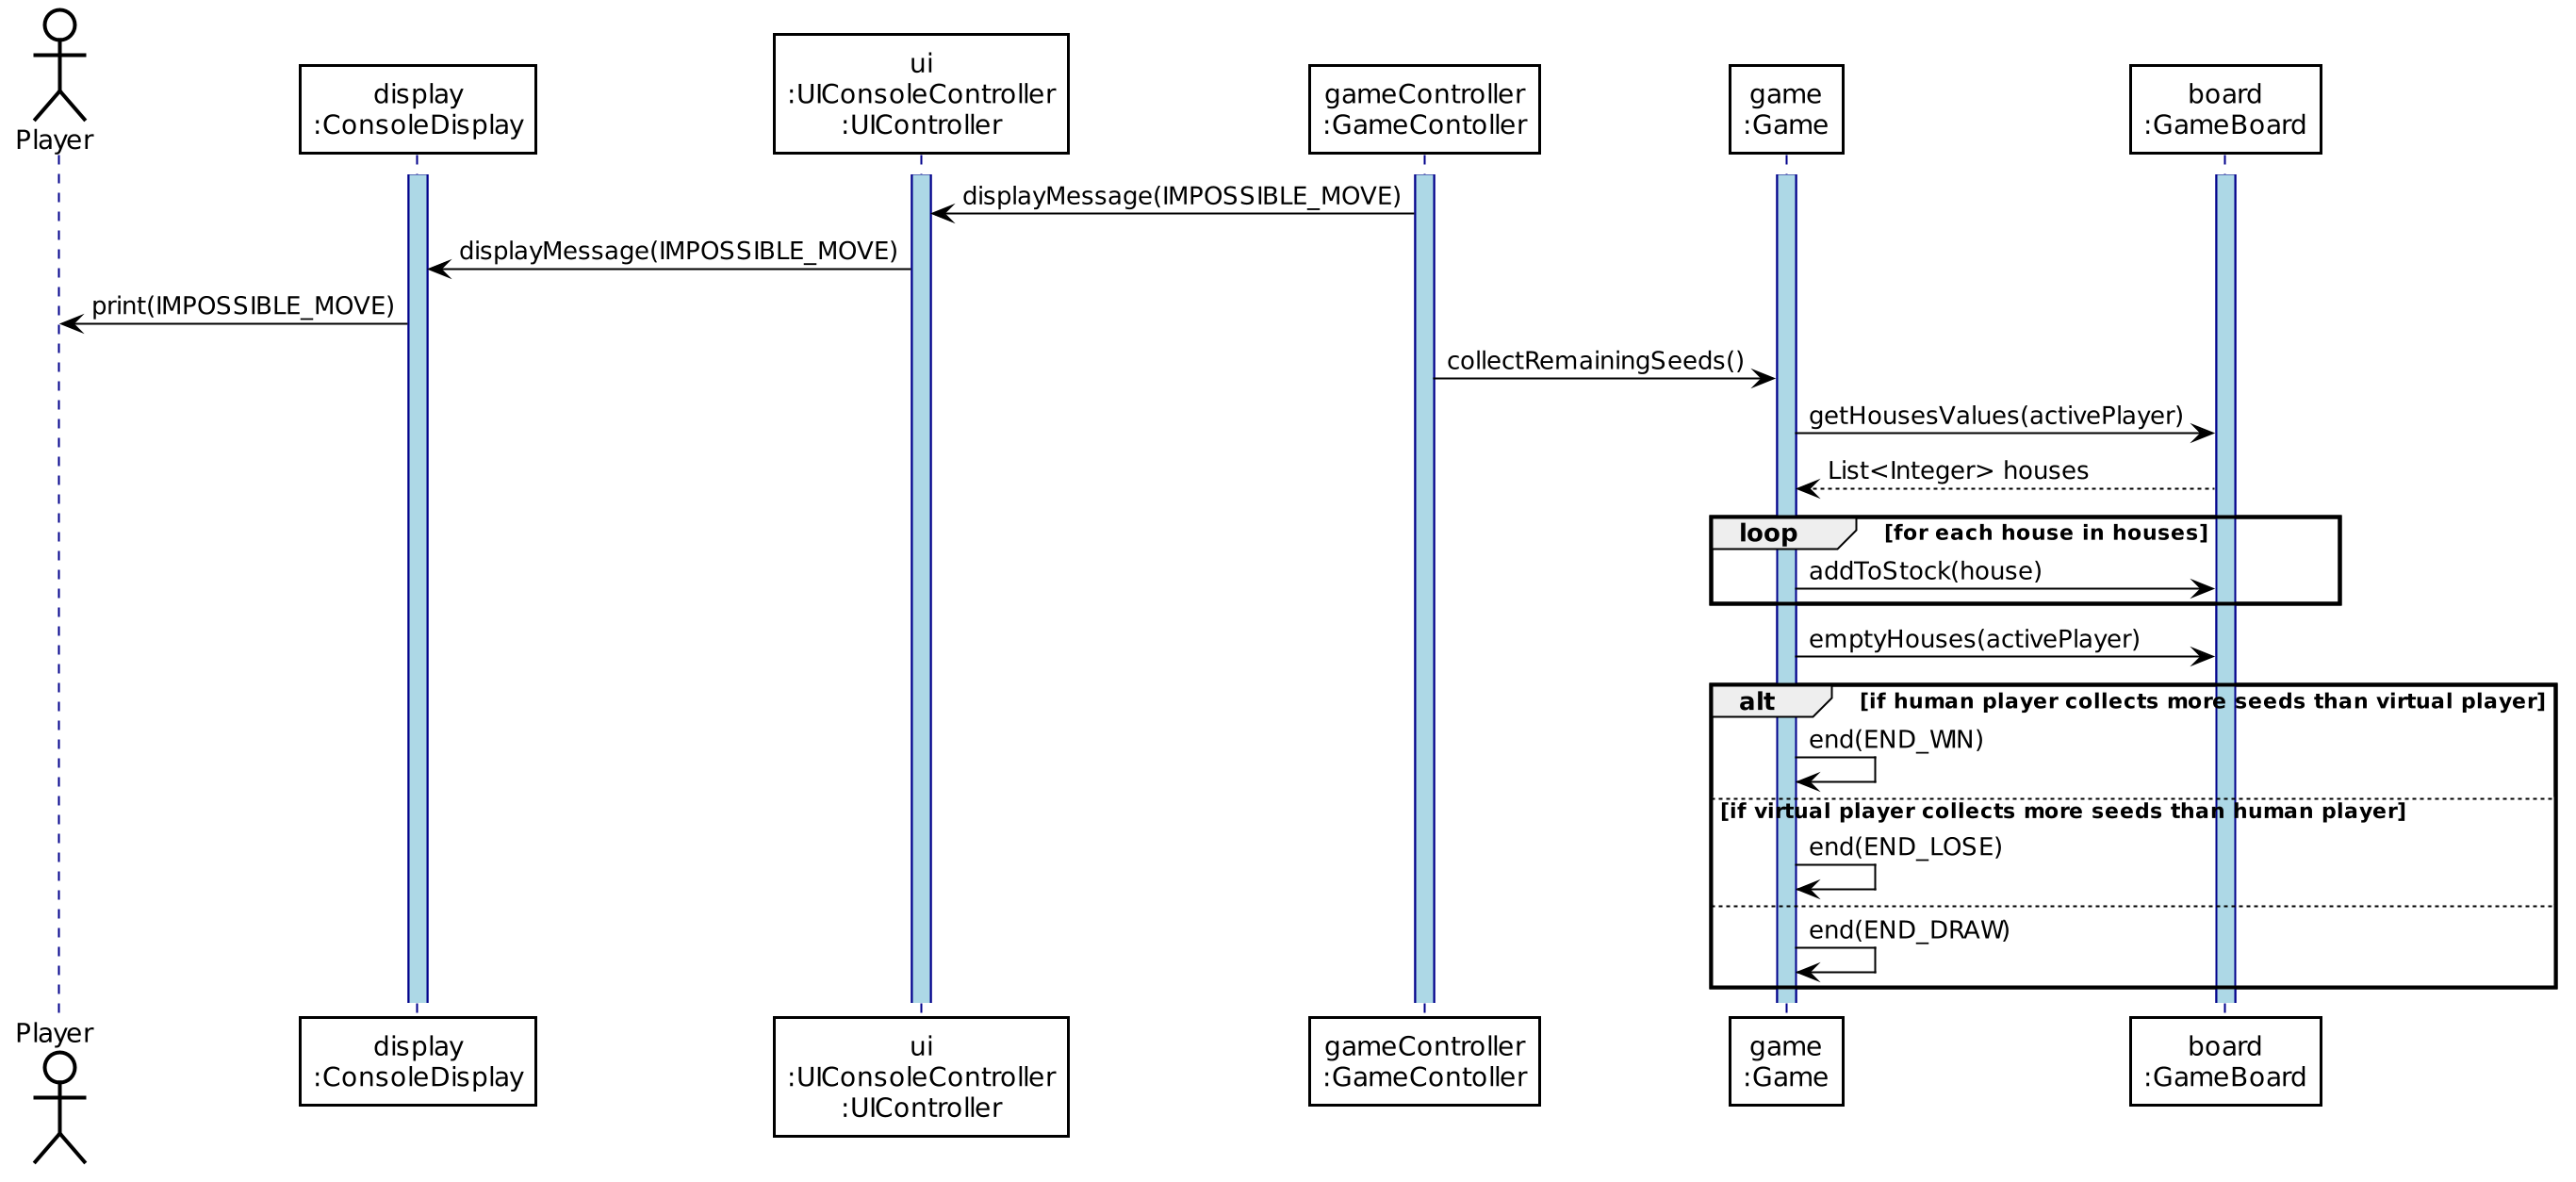
\includegraphics[width=\linewidth]{./schemas/sequence5-end-impossible-move.png}
    \end{figure}

    \paragraph{}
    Lorsque plus aucun mouvement n'est possible, le joueur actif peut récolter les graines qui restent dans ses trous, le stock est mis à jour et le gagnant est défini en fonction du joueur qui a le plus de graines en réserve (ou match nul si les deux joueurs ont récolté le même nombre de graines).


    \newpage
    \section*{Conclusion}
    \label{sec:concl}
    \addcontentsline{toc}{section}{\nameref{sec:concl}}

    \paragraph{}
    Afin de rendre les changements futurs plus faciles, j'ai implémenté un design pattern MVC avec la séparation des modèles, vues et contrôleurs. La logique du jeu est bien séparée de la logique d'interaction avec l'utilisateur. Les menus sont également définis de manière déclarative afin de pouvoir les affiner sans modifier la logique d'affichage.
    
    \paragraph{}
    Par contre, n'ayant pas d'expérience avec JavaFX, il m'a été difficile de prévoir avec le jeu en console ce qui pourrait être réutilisé dans le version suivante du jeu. Pour cette raison, l'interface \textbf{ConsoleUI} sera très probablement amenée à être modifiée.


\end{document}